\documentclass[11pt]{article}
\usepackage[margin=1in]{geometry}
\usepackage{setspace}
\usepackage{iftex}
\usepackage{amsmath,amssymb}
\usepackage{graphicx}

\ifPDFTeX
  \usepackage[T1]{fontenc}
  \usepackage{newtxtext,newtxmath}
\else
  \usepackage{fontspec}
  \setmainfont{Times New Roman}
\fi

\setstretch{1.0}
\setlength{\parskip}{0.4em}
\setlength{\parindent}{0pt}
\pagenumbering{gobble}

\begin{document}

\begin{titlepage}
\centering
\vspace*{1in}
{\LARGE \textbf{Quantum-Enhanced Strategic Siting of Energy Storage and Microgrids} \par}
\vspace{0.35in}
{\large \textit{Global Industry Challenge (GIC) 2026} \par}
\vspace{0.5in}
{\large Date: \today \par}
\vspace{0.25in}
\centering
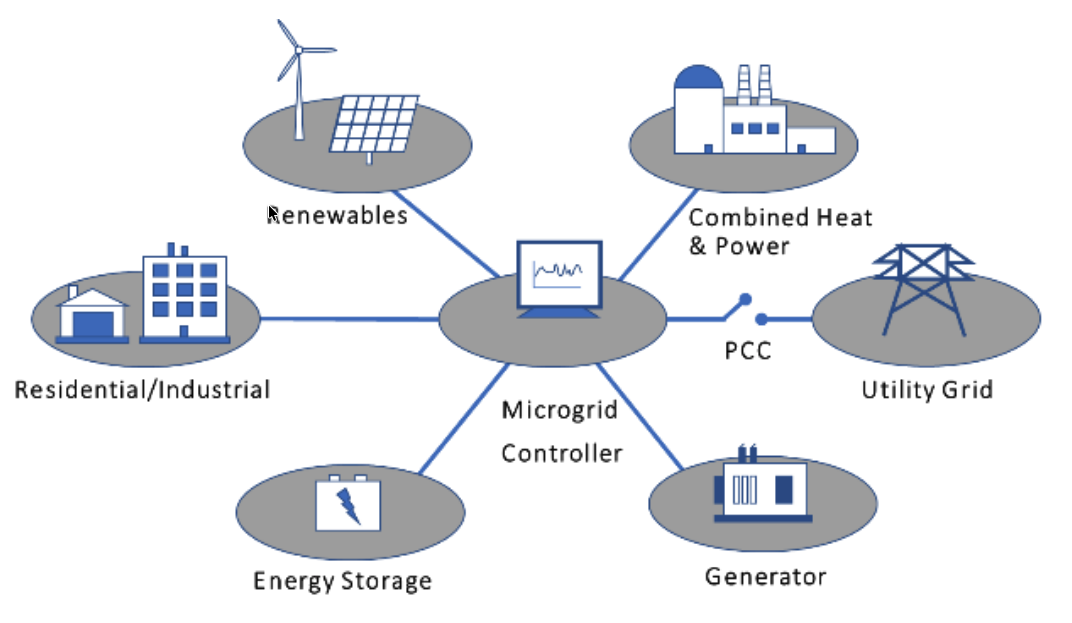
\includegraphics[width=0.80\textwidth]{../img/microgrid_components.png}
\vspace{0.25em}

{\footnotesize Figure 1: Microgrid architecture and components. Source: S. Atcitty, U.S. Department of Energy presentation.\par}
\vfill
{\large \textbf{Team Name} \par}
\vspace{0.25in}
\begin{tabular}{lll}
Name & Profession & Email \\
\hline
Niraj Venkat & MS/MBA Student and Researcher & venkatn93@gmail.com \\
\end{tabular}
\vspace*{0.6in}
\end{titlepage}

\noindent\textbf{Strategic Context}\\
This Phase 1 concept targets the fundamental computational bottleneck in grid modernization: solving large-scale mixed-integer nonlinear programming (MINLP) instances that determine where energy storage and microgrids should be deployed, how large they should be, and how they should operate under uncertainty. The candidate portfolio must satisfy nonlinear AC power-flow physics, contingency constraints, and multi-scenario cost and resilience trade-offs. We therefore frame the problem as a quantum-accelerated planning workflow that can explore feasible infrastructure portfolios faster than classical enumeration while preserving utility-grade validation.

\noindent\textbf{Proposed Solution Architecture}\\
We map the discrete planning layer into Quadratic Unconstrained Binary Optimization (QUBO) and Ising Hamiltonian formulations so that binary siting, sizing, and topology decisions become native inputs to quantum search. Continuous dispatch variables, AC feasibility, and reliability constraints remain on classical solvers. This separation keeps the hardest combinatorial search in the quantum loop while preserving full-fidelity power-system validation in the classical loop, which is essential for a Phase 1 prototype that must already be anchored to utility test systems.

\noindent\textbf{Hybrid Optimization Workflow}\\
The iteration follows a Hybrid Quantum-Classical Benders Decomposition (HQCBD) workflow. Rather than a single-objective QUBO only, we use a QAMOO-style multi-objective master in which weighted graph objectives are sampled and refined across scenarios:
\begin{align}
\max_{x,e}\quad & \mathbf{\lambda}^{\top}\mathbf{f}(x) = \sum_{k=1}^{m} \lambda_k f_k(x),
\qquad \sum_{k=1}^{m}\lambda_k = 1,\ \lambda_k\ge 0, \\
f_k(x) &= \sum_{(i,j)\in E_k} w_{ij}^{(k)} e_{ij},
\quad x_i\in\{0,1\},\ e_{ij}\in\{0,1\},
\end{align}
with cut variables \(e_{ij}\) linked to partition binaries by standard linear constraints. For scenario \(\omega\in\Omega\), feasibility is enforced classically through AC constraints and operating limits. We then sample either weighted-sum or epsilon-constraint subproblems,
\begin{equation}
\max_x\ \sum_{k=1}^{m} c_k f_k(x)
\quad\text{s.t.}\quad
f_j(x)\ge\epsilon_j^{(\omega)}\ \forall j,
\end{equation}
to enrich Pareto diversity before embedding into Ising form,
\begin{equation}
H_{\mathrm{cost}}(c)=\sum_{\langle i,j\rangle} h_{ij}(c) Z_i Z_j + \sum_i h_i(c) Z_i,
\end{equation}
and executing QAOA layers for candidate generation. Infeasible or weak candidates generate feasibility and optimality cuts,
\begin{equation}
\theta \le \lambda^{\top}f\!\left(x^{(s)}\right)-\rho_s, \qquad s=1,\dots,S,
\end{equation}
which are aggregated across scenarios to tighten the next master iteration.

\noindent\textbf{Technical Stack and Implementation Path}\\
Qiskit is the primary quantum programming layer for both simulation and hardware execution, matching the current QAMOO reference implementation and its IBM Runtime and Qiskit Aer execution path. We will use it to construct problem-specific ansatz templates, bind circuit parameters, manage shot budgets, and orchestrate the interface between quantum samples and classical optimization backends. The example QAMOO code informs the implementation style: QAOA-style gate blocks, graph-based problem encoding, and repeated evaluation of multiple candidate solutions. The Python side handles graph construction, scenario aggregation, and classical solvers such as AC feasibility checks and mixed-integer subproblem updates. The implementation path starts on reduced utility test systems and scales by increasing candidate sites, scenario count, and cut complexity while preserving the same software interfaces.

\noindent\textbf{Expected Phase 1 Deliverable and Validation}\\
Phase 1 delivers a working prototype that outputs ranked siting/sizing portfolios with scenario-aware operating summaries, AC-feasibility certificates, and Pareto trade-off reports. Validation compares portfolio quality, iteration efficiency, and solution diversity against classical baselines on the same reduced instances, including weighted-sum and branch-and-bound style comparisons where appropriate\footnote{Primary reference for this challenge: Nature Machine Intelligence article, \"https://www.nature.com/articles/s43588-025-00873-y\".}. The expected outcome is not full deployment, but clear evidence that the hybrid workflow can explore higher-quality candidate sets per planning cycle and expose a usable path toward larger planning studies.

\noindent\textbf{Conclusion}\\
The proposed approach positions quantum methods as a targeted accelerator inside an existing planning pipeline, not as a replacement for grid-physics modeling. By combining Qiskit-based quantum search with rigorous classical feasibility analysis and multi-objective scenario aggregation, the team can move from concept to code quickly and establish a credible path to larger, decision-relevant grid-planning studies.

\end{document}
